\documentclass[aspectratio=169]{beamer}
\usepackage{graphicx} % Required for inserting images

\usepackage{armtex}
\usepackage{amsmath}
\usepackage{amsthm}
\usepackage{tikz}
% \usepackage{xcolor}

% \usepackage[usenames,dvipsnames]{xcolor}
\usepackage{algorithm}
\usepackage{algpseudocode}
\usepackage{array}
\usepackage{longtable}
\usepackage{booktabs}
\makeatletter
\def\thmhead@plain#1#2#3{%
  \thmname{#1}\thmnumber{\@ifnotempty{#1}{ }\@upn{#2}}%
  \thmnote{ {\the\thm@notefont#3}}}
\let\thmhead\thmhead@plain
\makeatother

\newcommand{\red}[1]{\textcolor{red}{#1}}
\newcommand{\blue}[1]{\textcolor{blue}{#1}}
\newcommand{\yellow}[1]{\textcolor{yellow}{#1}}
\newcommand{\violet}[1]{\textcolor{violet}{#1}}
\newcommand{\orange}[1]{\textcolor{orange}{#1}}
\newcommand{\green}[1]{\textcolor{green}{#1}}

% ----------------------------\

\usepackage{amsmath}
% \beamertemplatenavigationsymbolsempty

\usetheme{Malmoe}

%gets rid of bottom navigation bars
\setbeamertemplate{footline}[frame number]{}

% %gets rid of bottom navigation symbols
\setbeamertemplate{navigation symbols}{}

%gets rid of footer
%will override 'frame number' instruction above
%comment out to revert to previous/default definitions
\setbeamertemplate{footline}{}

\title{Դեմստեր-Շաֆերի տեսության վրա հիմնված մեկնաբանելի ալգորիթմ}
\author{Հայկ Թարխանյան, Աշոտ Հարությունյան}
\date{\today}

\begin{document}

\begin{frame}
  \titlepage
\end{frame}

\begin{frame}
{\small\tableofcontents}
\end{frame}

% \begin{frame}{Նշում}
%     Դիպլոմայինը անգելերով է, սլայդերի մեջ որոշ մասեր նույնպես անգլերենով եմ թողել։ \\ \\ Հույս ունեմ խնդիր չի դա, եթե պետք է արագ կշտկեմ։ \\ \\Շնորհակալություն։    
% \end{frame}

\section{Հիմնական խնդիրը}
\subsection{Ձևակերպումը}
\begin{frame}{Մեկնաբանելիության դերը մեքենայական ուսուցման(ՄՈւ) մեջ}
\begin{columns}
  \begin{column}{0.5\textwidth}
    \begin{itemize}
      \item Հաճախ բարձր ճշտությամբ մոդելների մոտ առկա է լինում վատ բացատրելի լինելու խնդիրը։
      \pause
      \item Բացատրելի մոդել ունենալու խնդիրը երբեմն կրիտիկական կարևորություն է ունենում, օրինակի համար եթե ՄՈւ ալգորիթմի շնորհիվ կայացնենք մարդուն վարկ տալ/չտալու որոշումը ապա որոշ երկրներում օրենքով պարտադրված ենք լինելու նաև այդ մարդուն մերժելու դեպքում տալ համապատասխան հիմնավորումը։
    \end{itemize}
  \end{column}
  \pause
  \begin{column}{0.5\textwidth}
    % \includegraphics[width=\textwidth]{"interp_over_power.jpg"}
    % \pause
    % \includegraphics[width=\textwidth]{"interp_over_power_accent.jpg"}
    \begin{overprint}
        \onslide<3>\includegraphics[width=\textwidth]{"interp_over_power.jpg"}
        \onslide<4>\includegraphics[width=\textwidth]{"interp_over_power_accent.jpg"}
    \end{overprint}
\end{column}  
\end{columns}
\end{frame}

\begin{frame}{Մեկնաբանելիություն ապահովող ալգորիթմներ}
Կա երկու մոտեցում։
\begin{itemize}
    \item Արդեն ունենալով մոդելի կանխագուշակությունները փորձել բացատրել մոդելի աշխատանքը։ \pause
        \begin{itemize}
            \item \rm{LIME} (Local Interpretable Model-agnostic Explanations)
            \item SHAP (SHapley Additive exPlanations)
        \end{itemize}
    \pause
    \item Իսկզբանե բացատրելիությունը ներկառուցել մոդելի մեջ 
    \begin{itemize}
        \item Գծային ռեգրեսիա
        \item Մեր մոտեցումը (Դեմստեր-Շաֆերի տեսություն)
    \end{itemize}
\end{itemize}
\end{frame}


% \subsection{{\rm LIME (Local Interpretable Model-agnostic Explanations)}}
% \begin{frame}{{\rm LIME (Local Interpretable Model-agnostic Explanations)}}
%   \begin{itemize}
%     \item \textbf{Նպատակը:} Բացատրել կանխագուշակությունները ամեն կետի համար որոշակի լոկալ տիրույթում կլասիֆիկացիայի բացատրելի ալգորիթմ կիրառելով։ \pause
%     \item \textbf{Քայլերը:} 
%       \begin{enumerate} 
%         \item Գեներացնել կետեր տրված կետի որոշակի շրջակայքում և օգտագործել տրամադրած մոդելը պիտակներ ստանալու համար։ 
%         \item Կշիռ տալ այդ գեներացված կետերին ըստ նրանց և սկզբնական կետի Էվկլիդյան հեռավորության
%         \item Աշխատացնել բացատրելի մոդել (օրինակ գծային ռեգրեսիա), որը ստանալով այդ գեներացված կետերը կկանխագուշակի տրամադրած մոդելի պիտակները։
%       \end{enumerate}
%     \end{itemize}
% \end{frame}

% \begin{frame}{Մաթեմատիկական ձևակերպումը։}
%     \textbf{Մաթեմատիկական ձևակերպումը}
%     \begin{itemize}
%         \item Դիցուք \( x \)-ը կետ է որի համար պետք ա ստանանք մեկնաբանությունները և \( \xi \)-ն որևէ բացատրելի մոդել է (օրինակ գծային ռեգրեսիա).
%         \item Գեներացնել նոր կետերի \( Z \) բազմությունը \( \mathcal{N}(x, \sigma^2) \) բաշխումից որտեղ \( \sigma \)-ն կառավարում է թե որքան լոկալ ենք ուզում լինեն մեր բացատրությունները.
%         \item Լոկալ \( \xi \) մոդելին սովորացնում ենք մինիմիզացնել
%           \[
%           \mathcal{L}(f, \xi, \pi_x) = \sum_{z, z' \in Z} \pi_x(z) \left(f(z) - \xi(z')\right)^2
%           \]
%            ֆունկցիան որտեղ \( \pi_x(z) \) կշիռները սահմանող ֆունկրան է, \( f \)-ը մեզ տրամադրված մոդելը, իսկ \( Z \)-ը գեներացված կետերի բազմությունն է.
%     \end{itemize}
%     \textbf{Մեկնաբանումը:} \( \xi \) մոդելի գործակիցները իրենցից ներկայացնելու ենք \( x \) կետի վրա տարբեր ատրիբուտների ազդեցությունները։
% \end{frame}

\begin{frame}
    \begin{center}
        \Huge Դեմստեր-Շաֆերի տեսություն
    \end{center}
\end{frame}

\section{Դեմստեր-Շաֆերի տեսություն (ԴՍՏ)}
\begin{frame}{Դեմստեր-Շաֆերի տեսություն (ԴՍՏ)}
    \begin{block}{ԴՍՏ-ի ընդհանուր նկարագիրը}
        Դեմստեր-Շաֆերի տեսությունը (նաև հայտնի է որպես {\rm theory of belief functions}) մաթեմատիկական գործիք է որը մեզ թույլ է տալիս պնդումներ անել անորոշություն պարունակով պրոցեսների վերաբերյալ։ 
            \vspace{0.5cm}
            \\
        \pause
        Հիմնական կարևորությունը կայանում է պատահույթների {\rm "plausability"}-ն գնահատելու մեջ։     \vspace{0.5cm}
        % \pause
        % ԴՍՏ-ն կարող ենք դիտարկել որպես Բայեսի տեսության ընդհանրացում։
        
    \end{block}
\end{frame}


\subsection{{\rm Mass Assignment} ֆունկցիաներ}
\begin{frame}{{\rm Mass Assignment Function (MAF)}}
  \begin{itemize}
    \item \textbf{Մաթեմատիկական ձևակերպումը:}
      \begin{itemize}
        \item Դիցուք \( X \)-ը պատահույթների բազմությունն է, որը հայտնի է որպես {\rm frame of discernment} \pause
        \item {\rm Mass assignment function} \( m \)-ը ֆունկցիա է որոշված $X$-ի ենթաբազմությունների բազմության՝ \( 2^X \) վրա այնպես որ՝
          \[
          m : 2^X \rightarrow [0, 1]
          \]
        \pause
        \item Տեղի ունեն հետևյալ պայմանները։
          \begin{enumerate}
            \item \( m(\emptyset) = 0 \) (Դատարկ բազմությունը կշիռ չունի)
            \item \( \sum\limits_{A \subseteq X} m(A) = 1 \) (Կշիռների գումարը միշտ 1 է)
          \end{enumerate}
      \end{itemize}
  \end{itemize}
\end{frame}

\begin{frame}{{\rm MAF}-ի օրինակներ}
\begin{itemize}
    \item Պատկերացնենք որ ազնիվ կոպեկ ենք նետում, կլասիկ հավանականային մոդելի դեպքում սա կարող ենք արտահայտել որպես $P(\{heads\}) = (\{tails\}) = 0.5$, ԴՍՏ մոդելի դեպքում էլ կլինի $P(\varepsilon) = 0, P(\{heads\}) = (\{tails\}) = 0.5, P(\{heads, tails\}) = 0$:
    \pause
    \item Իսկ եթե կոպեկը անարդար լիներ կլասիկ մոտեցմանբ ոչմի բան չէինք կարող պնդել, մինչդեռ ԴՍՏ-ով կարող ենք ասել որ $P(\varepsilon) = 0, P(\{heads\}) = (\{tails\}) = 0, P(\{heads, tails\}) = 1$:
    \pause
    \item Օրինակ որտեղ կարող է շողալ ԴՍՏ-ն հետևայլն է։ Պատկերացնենք ինչ-որ մարդ իր կողքով անցնող մեքենա է տեսել և անում է հետևյալ պնդումը։ 
    \begin{enumerate}
        \item Մեքենայան կամ սև էր կամ շականակագույն, ամեն դեպքում ոնց-որ թե սև էր, բայց դե գուցե սխալվում եմ։ 
        Այս դեպքում {\rm MAF}—ը կարող է ունենալ այսպիսի տեսք։ $m(\{\varnothing\}) = 0.1, m(\{ black\}) = 0.4, m(\{ brown\}) = 0.3, m(\{ black, brown\} = 0.2$
    \end{enumerate}
    % same as prob. dist. func
\end{itemize}
\end{frame}

\subsection{{\rm Belief} և {\rm Plausibility}}
\begin{frame}{{\rm Belief} և {\rm Plausibility}}
    \begin{block}
         $\forall  A  \in X $
          \[
          Bel(A) = \sum_{B \subseteq A} m(B)
          \]
        \[
          Pl(A) = \sum_{B \cap A \neq \emptyset} m(B)
          \]
            \[
            Bel(A) \le P(A) \le Pl(A)
            \]

    Նախորդ օրինակի դեպքում սև մեքենայի համար կունենանք՝
    $m(\{\varnothing\}) = 0.1, m(\{ black\}) = 0.4, m(\{ brown\}) = 0.3, m(\{ black, brown\} = 0.2$ \\
    $A$ = սև, $B$ = շակագույն
          \[
        Bel(A) = m(A) = 0.4 \]
        \[
        Pl(A) = m(A) + m(\{A, B\}) = 0.4 + 0.2 = 0.6
          \]
    \end{block}
    % \begin{block}
    
    % \end{block}
\end{frame}

% ԹՈՒԴՈՒ
\subsection{Դեմստերի օրենք}
\begin{frame}{Դեմստերի օրենք}
\begin{itemize}
  \item Դեմստերի օրենքը կիրառվում է \(m_1\) և \(m_2\) {\rm MAF}-ը միավորելու համար.
  \item \textbf{Բանաձևը}
    \begin{equation*}
      m_f(A) = m_1(A) \oplus m_2(A) = \frac{1}{1 - K} \sum_{B \cap C = A} m_1(B) m_2(C)
    \end{equation*}
    \pause
  \item \textbf{Անհամաձայնության չափ \(K\):}
    \begin{equation*}
      K = \sum_{B \cap C = \emptyset} m_1(B) m_2(C)
    \end{equation*}
    \pause
  \item Եթե $K=1$ հանգում ենք զրոյի բաժանման խնդրի։
  \end{itemize}
\end{frame}

\begin{frame}{}
    \begin{block}{Աբելյան կիսախումբ}
\begin{itemize}
  \item Դիցուք \(M_{\Omega}\)-ն բոլոր հնարավոր {\rm MAF}-երի բազմությունն է սահմանված \(\Omega\) պատահույթների բազմության վրա: \pause
  \item \((M_{\Omega}, \oplus)\)-ն հանդիսանում է Աբելյան կիսախումբ: 
  \begin{itemize}
    \item Ասոցատիվություն \( m_1 \oplus (m_2 \oplus m_3) = (m_1 \oplus m_2) \oplus m_3 \)
    \item Կոմուտատիվություն \( m_1 \oplus m_2 = m_2 \oplus m_1 \)
  \end{itemize}
\end{itemize}
\end{block}
\pause
\begin{block}{Զրոյացնող ({\rm Absorbent}) և միավոր էլեմենտ}
\begin{itemize}
  \item Կլանող էլեմենտ
  \begin{itemize}
    \item Դիցուք \(C_A : 2^X \to [0, 1]\) այնպես որ \(C_A(A) = 1\) և \(\forall Y \neq A, C_A(Y) = 0\).
    \item Ապա \(m \oplus C_A = C_A\).
\pause
  \end{itemize}
  \item Միավոր էլեմենտ:
  \begin{itemize}
    \item Դիցուք \(U : 2^X \to [0, 1]\) այնպես որ \(U(X) = 1\) և \(\forall Y \neq X, U(Y) = 0\).
    \item Ապա \(m \oplus U = m\).
  \end{itemize}
\end{itemize}
\end{block}

\end{frame}


\section{Ներկայիս մոտեցումը}

\begin{frame}
    \begin{center}
        \Huge Ներկայիս մոտեցումը
    \end{center}
\end{frame}

\begin{frame}{Ներկայիս մոտեցումը}
    Կանխագուշակություն անելու համար՝
\begin{enumerate}
    \item Տվյալների համար գեներացվում է օրենքների $RS$ բազմությունը
    \item Ամեն օրենքին համապատասխանող $MAF$-ին սկզբնական արժեքներ ենք տրվում հետևյալ սկզբունքով։ Անորոշությունը (ամբողջ բազմությունը) ստանում է 0.8 կշիռ, և մնացած 0.2-ը պատահականորեն բաշխվում է $singletron$ էլեմենտների մեջ։
    \item Մուտքում ստանում ենք $x$ և՝
\end{enumerate}

\end{frame}

\begin{frame}
\begin{figure}
    \centering
    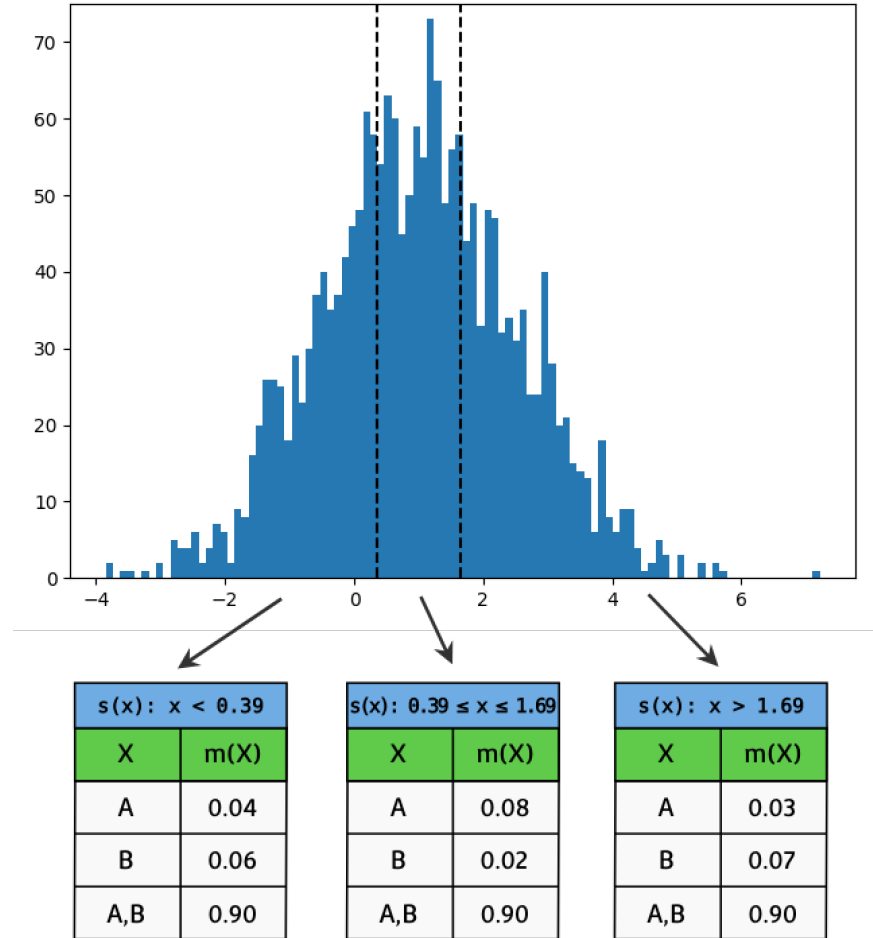
\includegraphics[width=0.45\linewidth]{image.png}
    \label{fig:enter-label}
\end{figure}
    
\end{frame}



\begin{frame}{Ներկայիս մոտեցումը}
\begin{align*}
\mathcal{M}_x &= \left\{ m \mid (m, s) \in RS \land x \right\} \\
m_f &= \bigoplus_{m \in \mathcal{M}_x} m \\
\hat{y} &= \underset{{\rm class}}{\mathrm{argmax}} \, {\rm Bel}(m_f)
\end{align*}

\end{frame}

% \begin{frame}{Օպտիմիզացիա}
%     Օգտագործում ենք $ADAM$ ալգորիթմը։
% \begin{align*}
% m_t &= \beta_1 m_{t-1} + (1 - \beta_1) \frac{dJ}{d\theta} \\
% v_t &= \beta_2 v_{t-1} + (1 - \beta_2) \left(\frac{dJ}{d\theta}\right)^2 \\
% \hat{m}_{t+1} &= \frac{m_t}{1 - \beta_1^t} \\
% \hat{g}_{t+1} &= \frac{v_t}{1 - \beta_2^t} \\
% \theta_{t+1} &= \theta_t - \frac{\alpha \hat{m}_{t+1}}{\sqrt{\hat{g}_{t+1}} + \varepsilon}
% \end{align*}
% \end{frame}

% where: TODO
% \begin{itemize}
%   \item \( m_t \) and \( v_t \) are estimates of the first moment (the mean) and the second moment (the uncentered variance) of the gradients, respectively.
%   \item \( \frac{dJ}{d\theta} \) is the gradient of the objective function \( J \) with respect to the parameters \( \theta \) for the current time step.
%   \item \( \beta_1 \) and \( \beta_2 \) are the exponential decay rates for the moment estimates.
%   \item \( \hat{m}_t \) and \( \hat{v}_t \) are bias-corrected versions of \( m_t \) and \( v_t \).
%   \item \( \alpha \) is the step size.
%   \item \( \epsilon \) is a small scalar used to prevent division by zero.
%   \item \( \theta_t \) are the parameters to be updated.
% \end{itemize}

\begin{frame}{Սխալանքի ֆունկցիա}
    \begin{block}{Միջին քառակուսային շեղում}
        \begin{equation}
MSE = \frac{1}{n} \sum_{i=1}^{n} \left\| y_i - \hat{y}_i \right\|^2
        \end{equation}
    \end{block}
    \begin{block}{{\rm Cross-Entropy}}
        \begin{equation}
        CE = - \frac{1}{n} \sum_{i=1}^{n} \sum_{j=1}^{k} y_{ij} \cdot \log(\hat{y}_{ij})
        \end{equation}
    
    \end{block}
        
\end{frame}
\begin{figure}
    \centering
    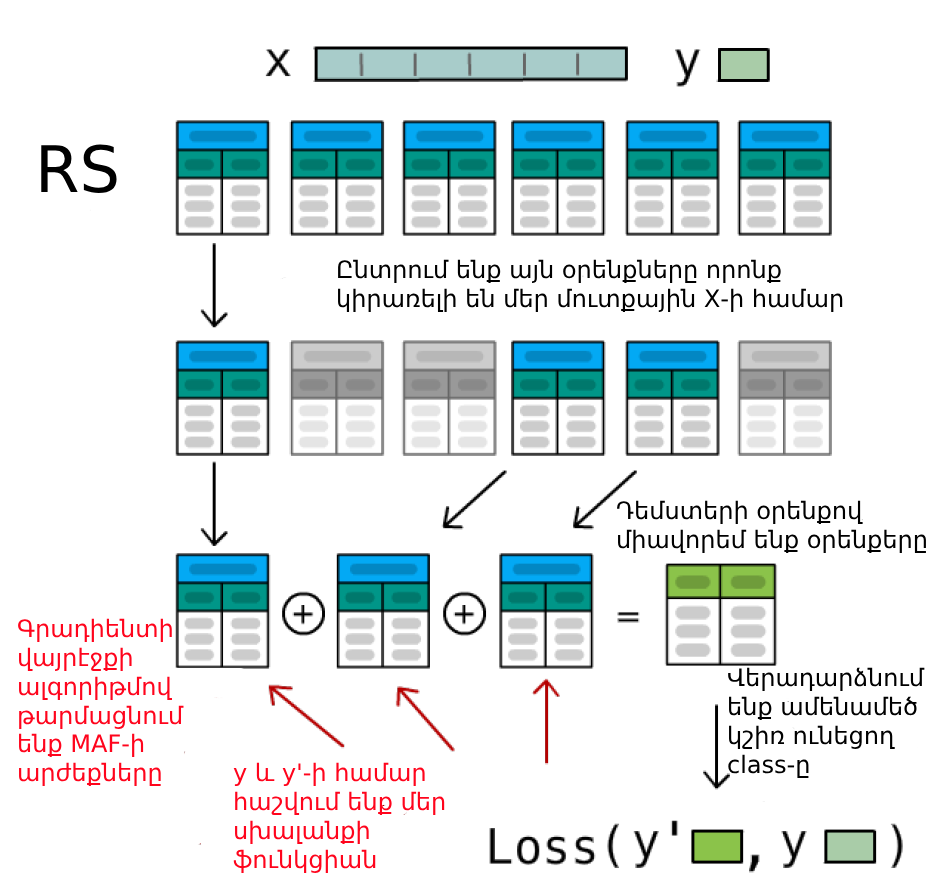
\includegraphics[width=0.55\linewidth]{dst_ill.png}
\end{figure}




\section{Մեր մոտեցումը}
\begin{frame}
    \begin{center}
        \Huge Մեր մոտեցումը
    \end{center}
\end{frame}
\subsection{{\rm KMeans}}
\begin{frame}
\begin{figure}
    \centering
    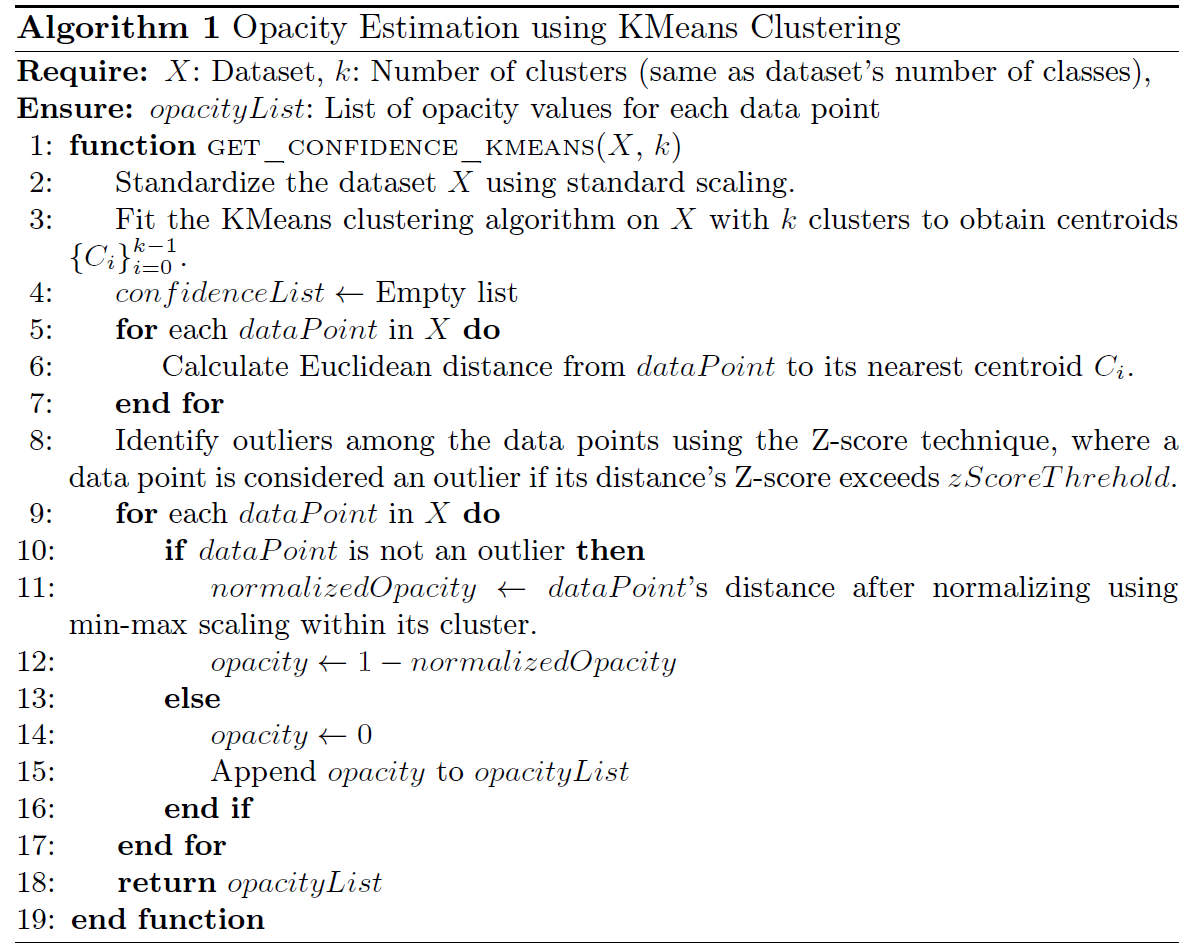
\includegraphics[width=0.68\linewidth]{alg_kmeans_opacity.png}
    \caption{Enter Caption}
    \label{fig:enter-label}
\end{figure}
\end{frame}

\begin{frame}
\begin{figure}
    \centering
    \includegraphics[width=0.78\linewidth]{kmeans_opactiy.png}
    \label{fig:enter-label}
\end{figure}
\end{frame}

\subsection{{\rm DBSCAN}}
\begin{frame}
\begin{figure}
    \centering
    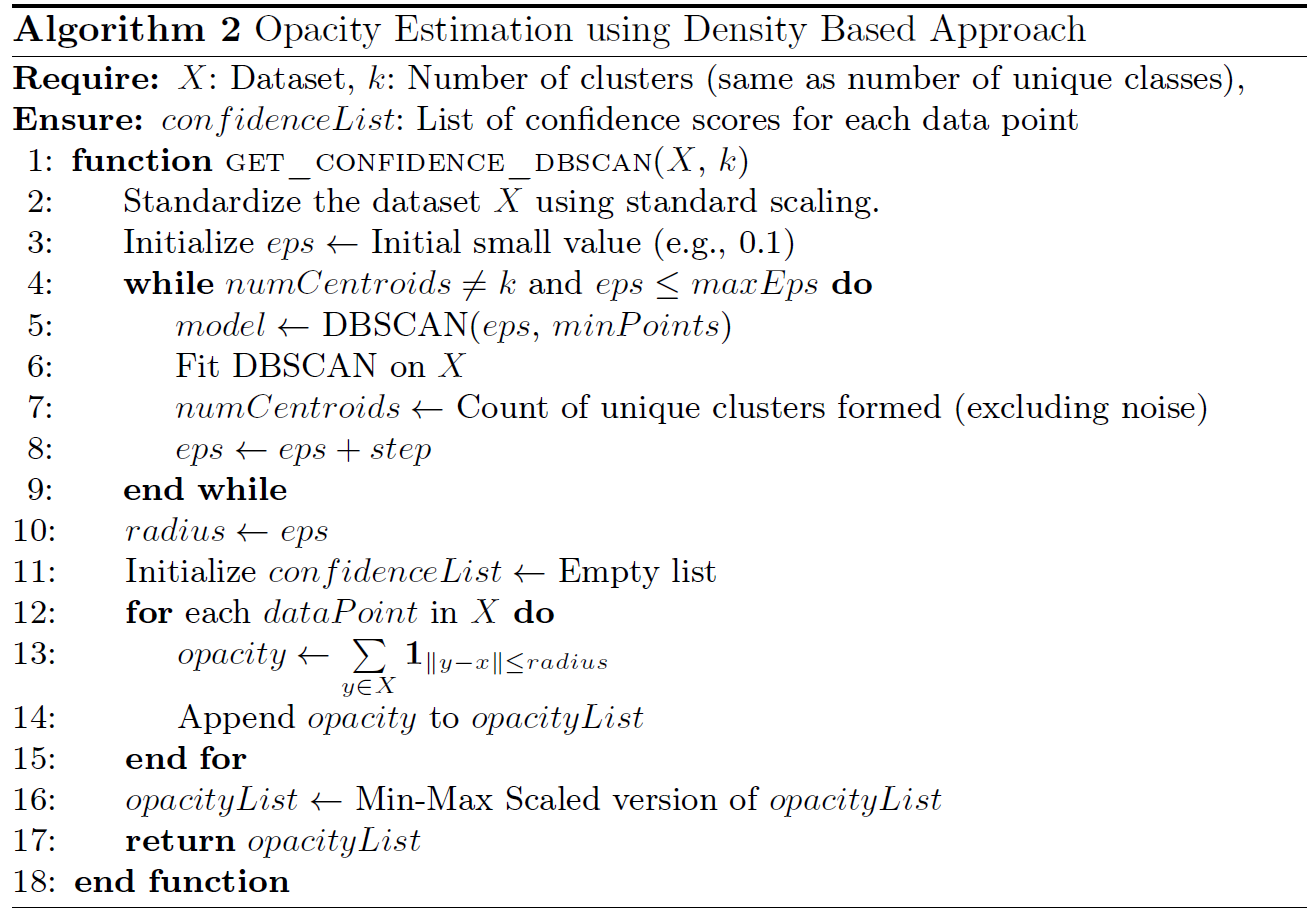
\includegraphics[width=0.75\linewidth]{alg_dbscan_opacity.png}
    \label{fig:enter-label}
\end{figure}
    
\end{frame}


\begin{frame}
\begin{figure}
    \centering
    \includegraphics[width=0.75\linewidth]{denisty_opactiy.png}
    \label{fig:enter-label}
\end{figure}
\end{frame}

\subsection{Օրենքի {\rm Confidence}-ի գնահատում}
\begin{frame}{Օրենքի {\rm Confidence}-ի գնահատում}

\begin{enumerate}
    \item Ընտրել միայն այն տողերը որոնք հետևում են օրենքին։ \pause
    \item Եթե ստացվող բազմությունը դատարկ է արտածել 0: \pause
    \item Հաշվել բազմության էլեմենտների {\rm Representativeness}-ների միջինը։ \pause
    \item Եթե բազմությունում առկա են տարբեր պիտակներով էլեմենտներ նվազեցնել ստացված արժեքը ըստ ամենատարածված պիտակի չափապաժնի։
\end{enumerate} 
\end{frame}


% \subsection{{\rm MAF}-ի ինիցալիզացիա}
% \begin{frame}{{\rm MAF Initialization}}
% \begin{block}
%     {\rm
%     In the Mass Assignment Function (MAF), we use the following values for initialization. Let $c = get\_confidence(rule)$ represent the confidence derived for a given rule. The label $l_{\text{mode}}$, which is the most frequently occurring label within the subset of data points covered by the rule, receives the confidence value $c$. The remaining mass, $(1 - c)$, is evenly distributed among all other labels present in the subset. Formally, for an element $l_i$ in the subset:
% \[
% m(l_i) = 
% \begin{cases} 
% c & \text{if } l_i = l_{\text{mode}}, \\
% \frac{1-c}{n-1} & \text{otherwise},
% \end{cases}
% \]
% where $m(l_i)$ denotes the mass assigned to label $l_i$, and $n$ is the total number of elements in the frame of discernment. 
% }
% \end{block}

% \end{frame}

\subsection{{\rm MAF}-ի ինիցալիզացիա}
\begin{frame}{{\rm MAF Initialization}}
\[
m(l_i) = 
\begin{cases} 
c & \text{եթե } l_i = l_{\text{{\rm mode}}}, \\
\frac{1-c}{n-1} & \text{մնացած դեպքերում},
\end{cases}
\]


\end{frame}




\section{Արդյունքներ}


\begin{frame}
    \begin{center}
        \Huge Արդյունքներ
    \end{center}
\end{frame}

\subsection{{Տվյալները}}
\begin{frame}{Տվյալները}
{\rm
\begin{longtable}{|>{\raggedright\arraybackslash}p{3cm}|c|c|>{\raggedright\arraybackslash}p{5cm}|}
\hline
\textbf{Dataset} & \textbf{Rows} & \textbf{Columns} & \textbf{Description} \\ \hline
\endfirsthead
\hline
\textbf{Dataset} & \textbf{Rows} & \textbf{Columns} & \textbf{Description} \\ \hline
\endhead
Brain Tumor & 3762 & 14 & Includes first-order and texture features with target levels. \\ \hline
Breast Cancer Wisconsin & 699 & 9 & Clinical reports detailing cell benignity or malignancy. \\ \hline
Gaussian & 500 & 3 & Two 2D Gaussian distributions generate this dataset. \\ \hline
Uniform & 500 & 3 & Uniform samples from [-5, 5], with class split by the sign of x. \\ \hline
Rectangle & 1263 & 3 & Points in [-1, 1]×[-1, 1], class determined by the y component's sign. \\ \hline
\end{longtable}
    }
\end{frame}

\subsection{Արագագործության և ճշգրտության վերլուծություն}
\begin{frame}{Արագագործության և ճշգրտության վերլուծություն}
\begin{figure}
    \centering
    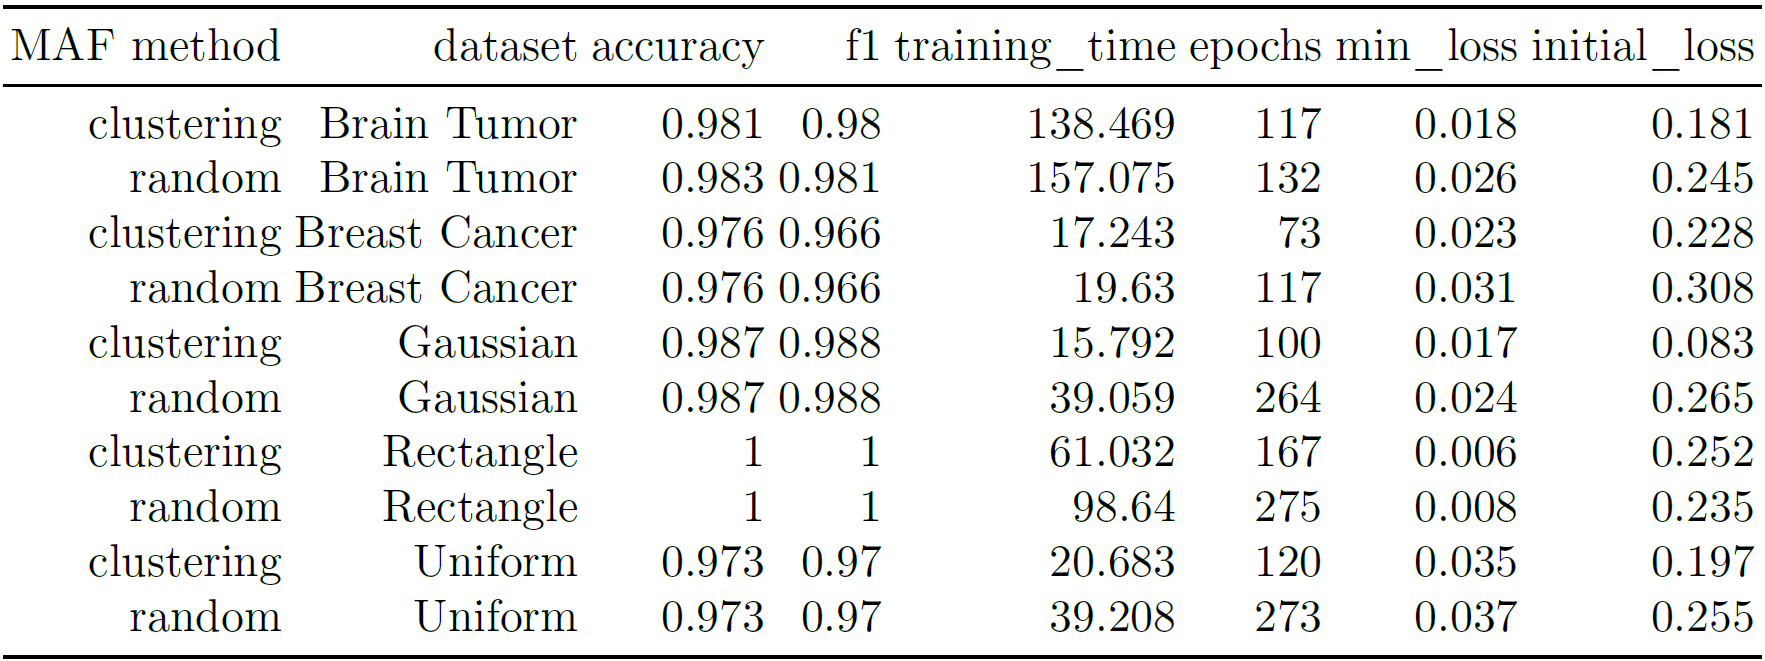
\includegraphics[width=0.95\linewidth]{acc_speedup_table.png}
    % \caption{Enter Caption}
    \label{fig:enter-label}
\end{figure}
\end{frame}

\begin{frame}
\begin{figure}
    \centering
    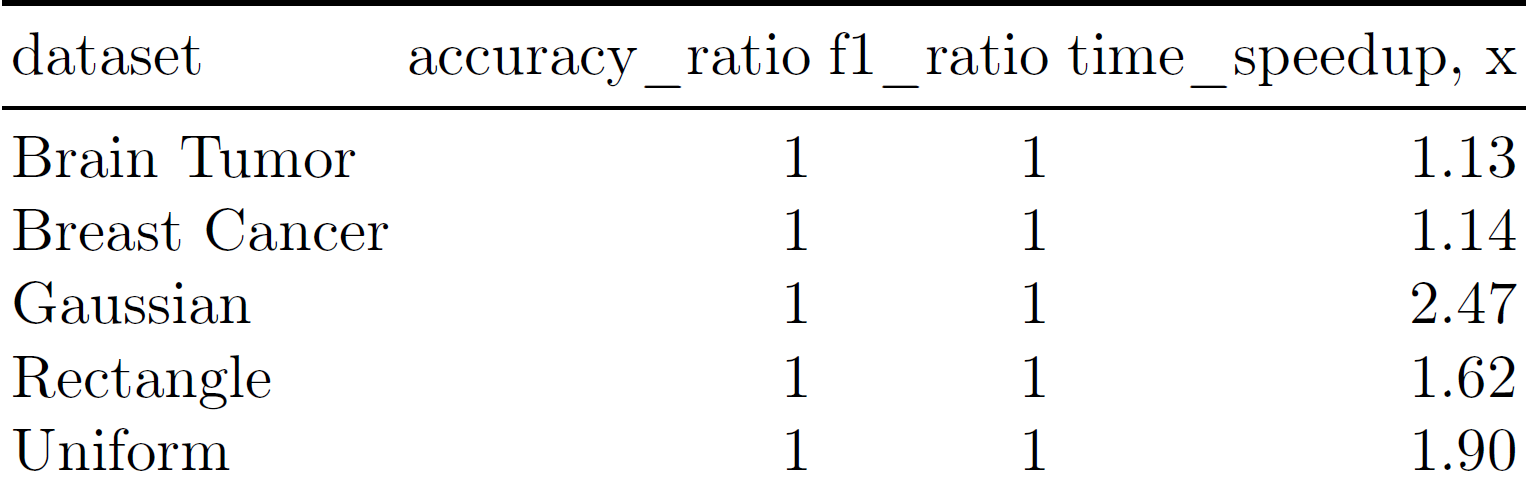
\includegraphics[width=1\linewidth]{speedup_groupby.png}
\end{figure}
\textbf{Արագության աճը միջինում - 1.65{\rm x}}
    
\end{frame}

\begin{frame}
    \begin{figure}
    \centering
    \begin{minipage}{0.49\textwidth}
        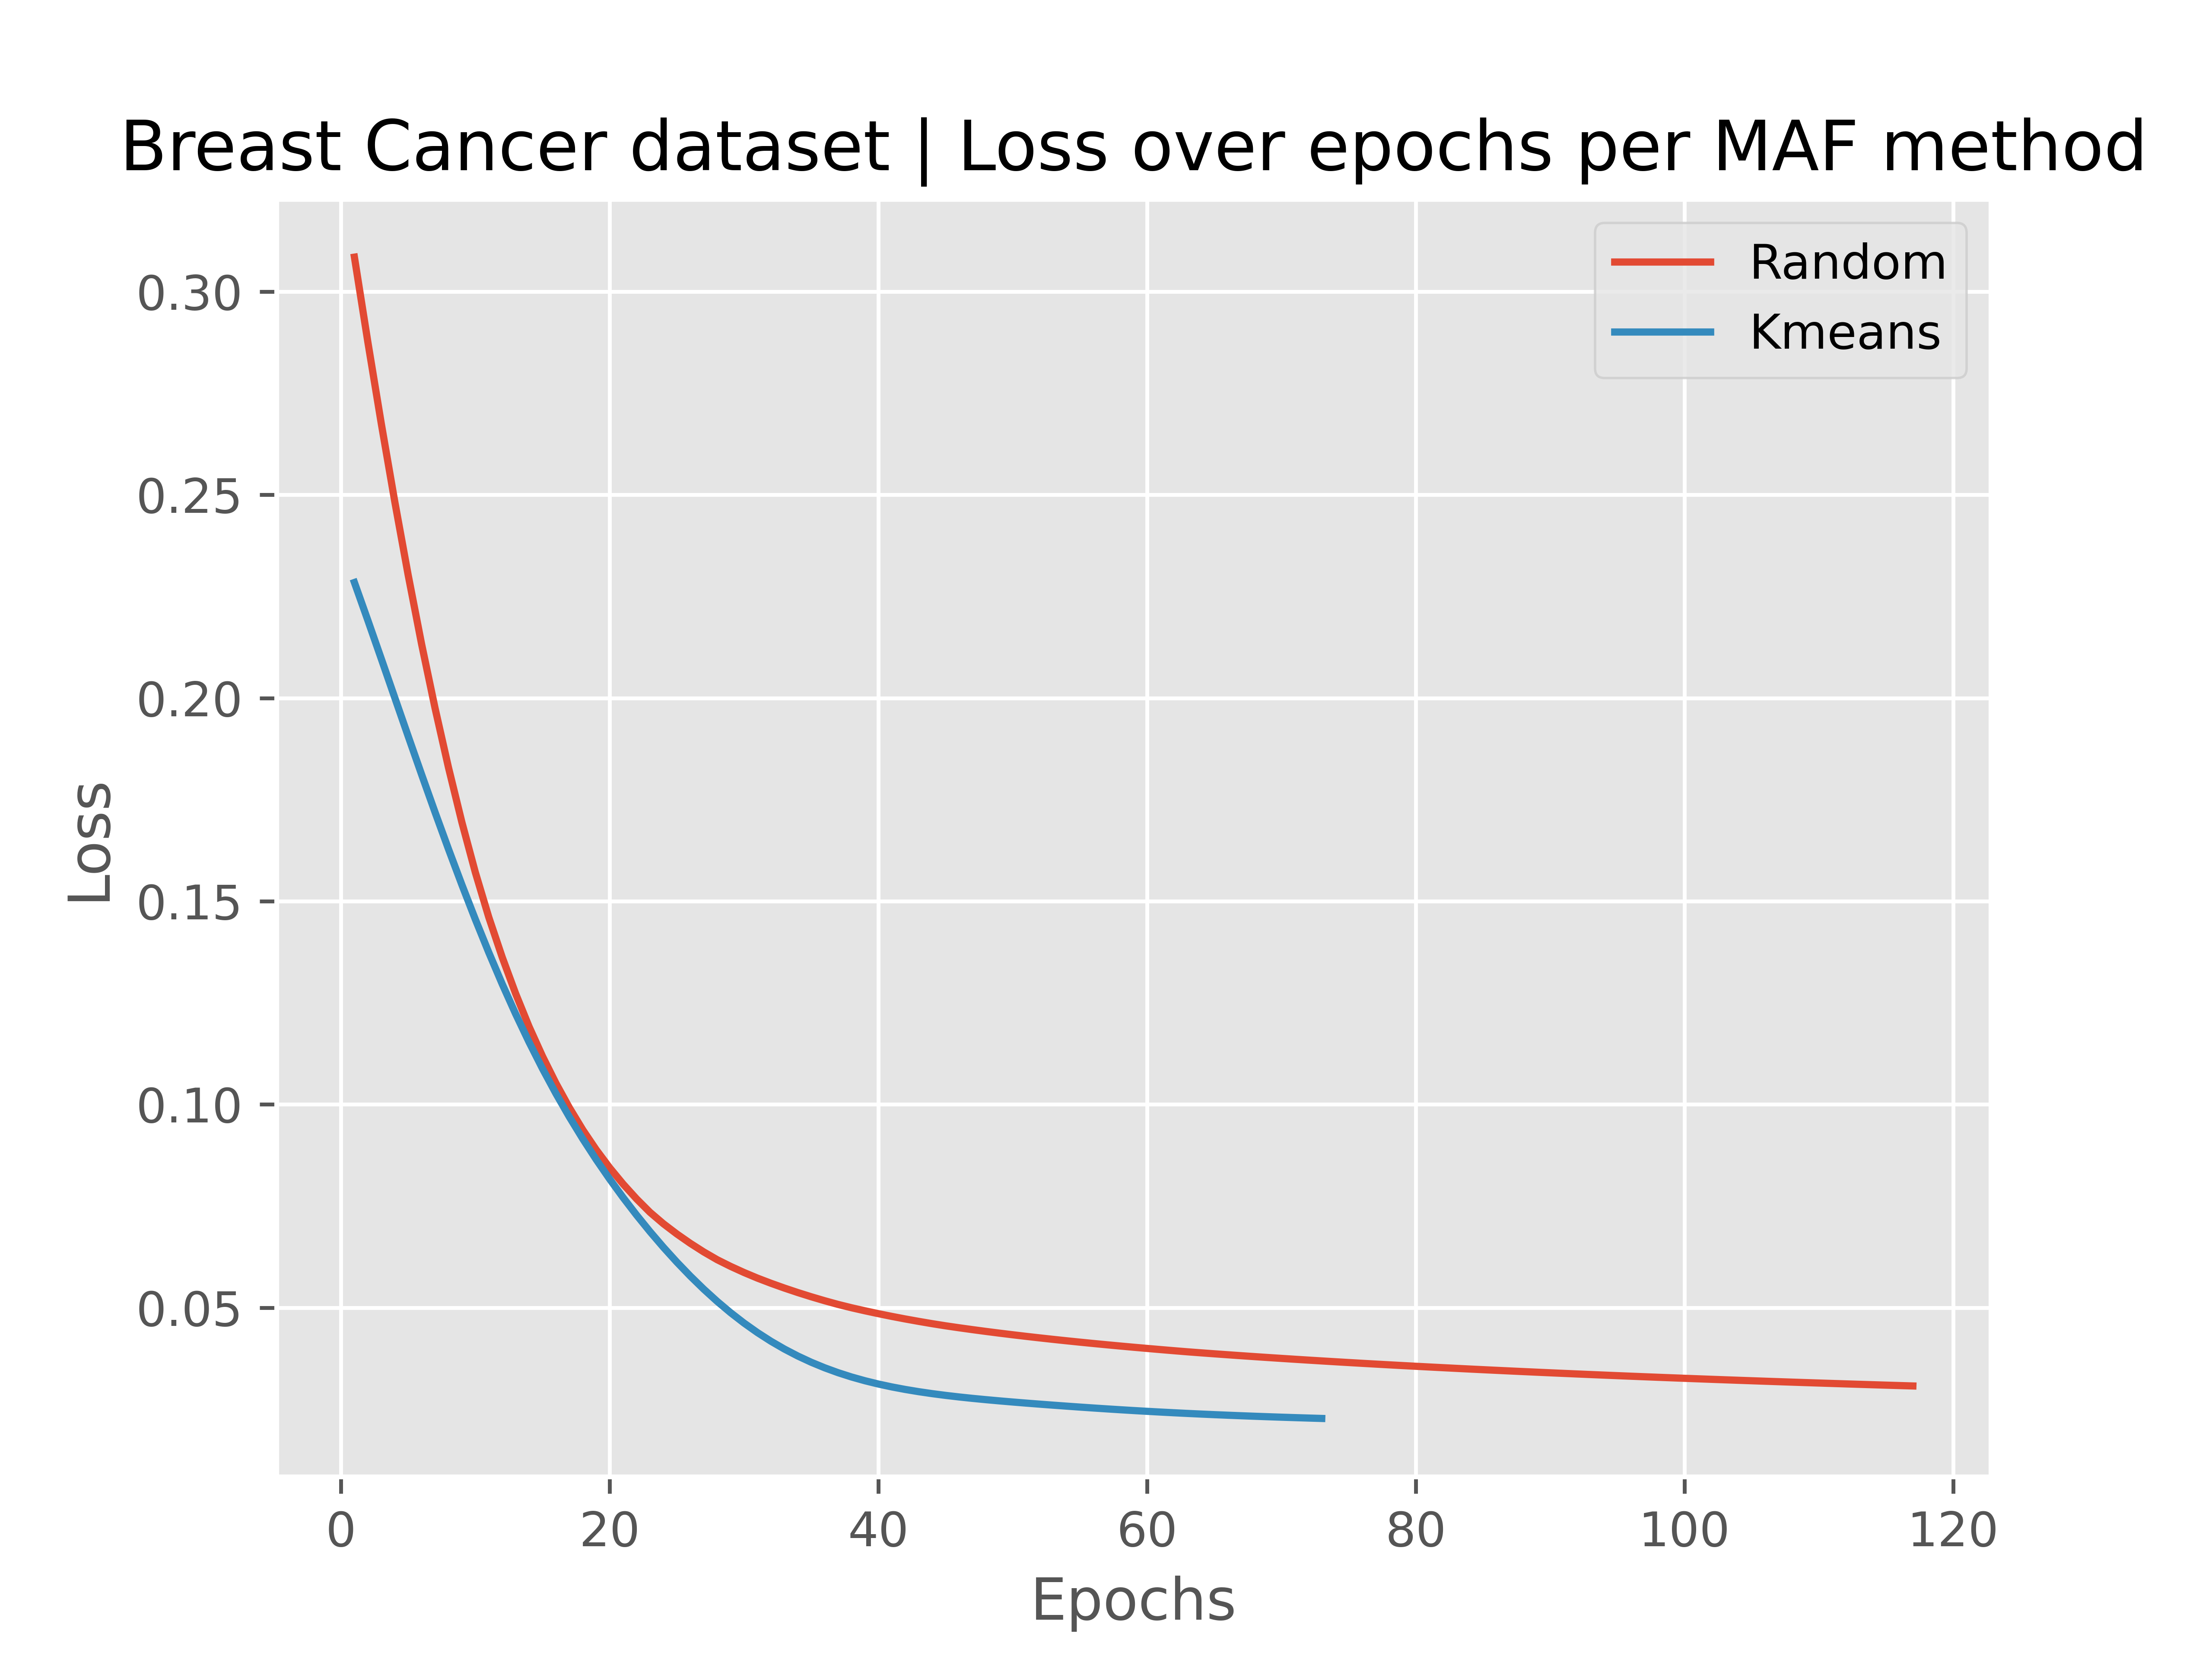
\includegraphics[width=\linewidth]{breast-cancer-wisconsin_loss.png} % First image
    \end{minipage}\hfill
    \begin{minipage}{0.49\textwidth}
        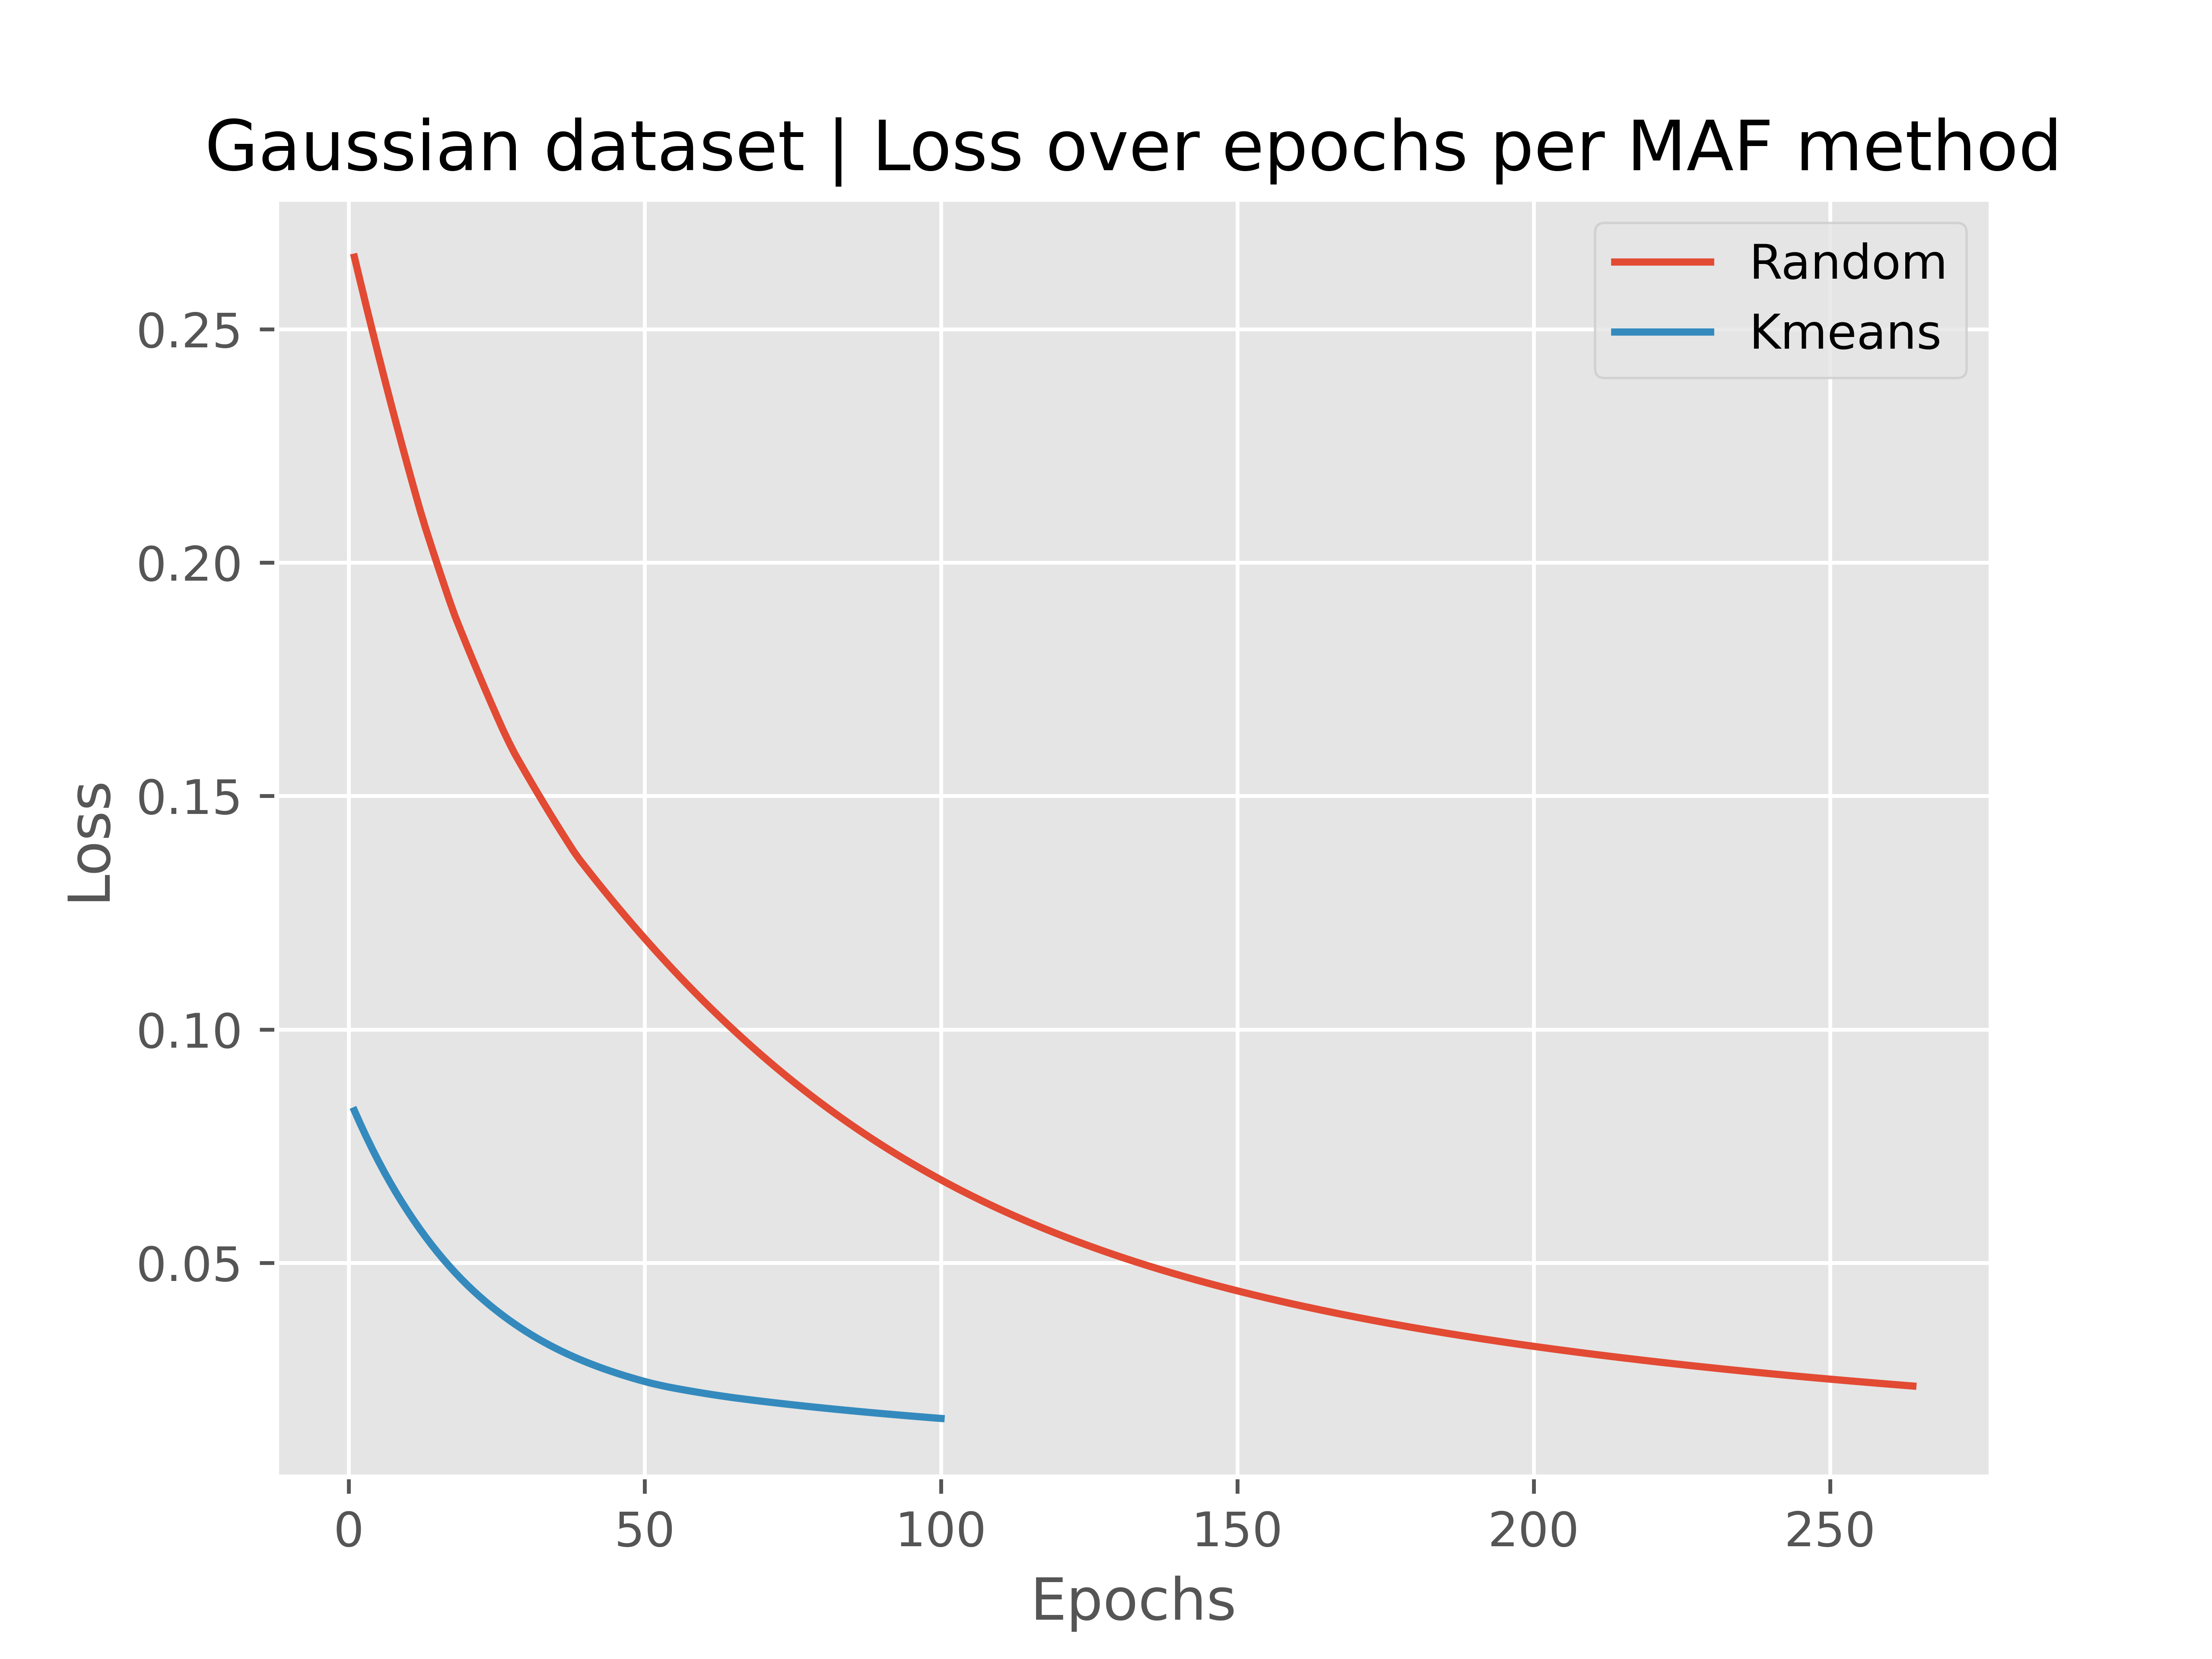
\includegraphics[width=\linewidth]{gaussian_df_loss.png} % Second image
    \end{minipage}
    \caption{Այս պատկերը ցուցադրում է {\rm MAF initialization}-ի հանգեցրած բարելավումները։ Մասնավորապես՝ ավելի լավ սկզբնակետ և ավելի քիչ իտերացիաներով զուգամիտում}
    \label{fig:side_by_side}
\end{figure}
\end{frame}

\subsection{Անորոշության վերլուծություն}
\begin{frame}{{\rm Անորոշության գնահատման ներկա մոտեցման բացթողումը}}
\begin{figure}
    \centering
    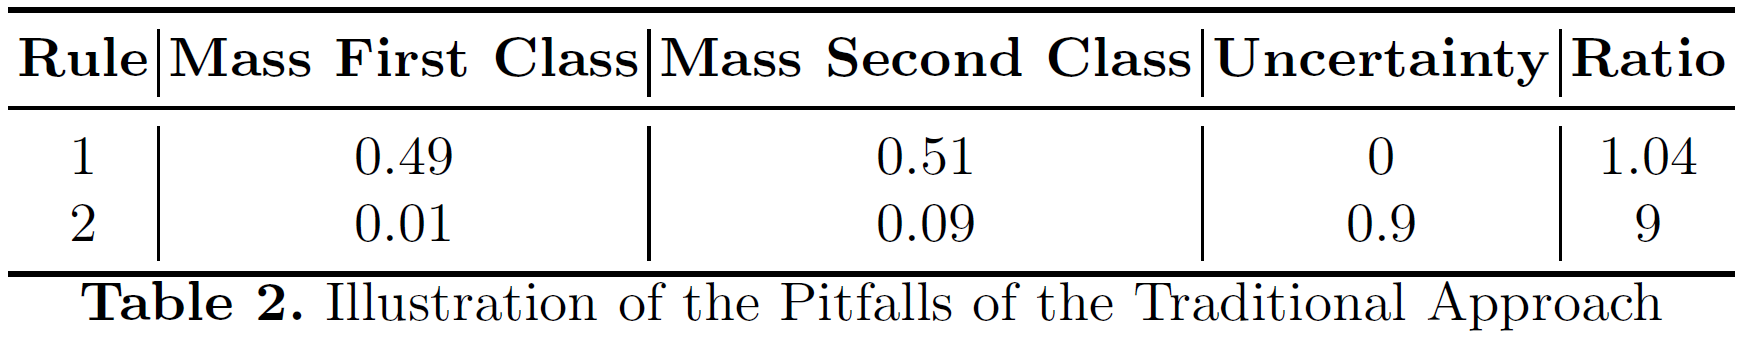
\includegraphics[width=1\linewidth]{pitfalls.png}
\end{figure}
\end{frame}

\begin{frame}
\begin{itemize}
\item \textbf{Անորոշության ուղղում}
    \[
    U' = 1 - U
    \]
    որտեղ \( U \)-ն սկզբնական անորոշությունն է.
    \pause
    \item \textbf{Հարաբերության նորմավորում}
    \[
    R' = \frac{R - \min(R)}{\max(R) - \min(R)}
    \]
    Որտեղ \( R \)-ը դա սկզբնական հարաբերությունն է (երկու կշիռների արժեքները իրար վրա բաժանելիս հայտարարիս գումարում ենք $\varepsilon=0.01$ զրոյի վրա բաժանումից խուսափելու համար)։ \( \min(R) \) և \( \max(R) \)-ը բոլոր օրենքների հարաբերությունների համապատասխանաբար մինիմումը և մաքսիմումն են։
    \pause
    \item \textbf{Հարմոնիկ միջինի հաշվարկ}
    \[
    H = \frac{2 \cdot U' \cdot R'}{U' + R'}
    \]
     
\end{itemize}
\end{frame}

\begin{frame}
\begin{figure}
    \centering
    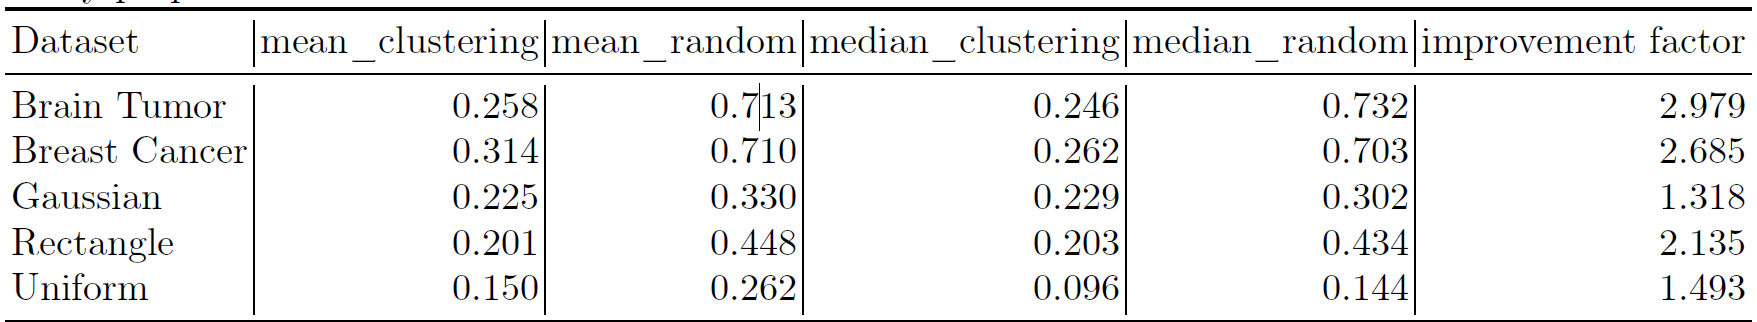
\includegraphics[width=1\linewidth]{unc_df.png}
\end{figure}
{\rm $improvement\_factor$}-ը սահմանված է որպես $median\_random$-ի և $median\_clustering$-ի հարաբերություն. \\ \pause
Մեր մոտեցումը հանեգնում է  անորոշության միջինում \textbf{2.12} անգամ նվազեցման։
    
\end{frame}

\begin{frame}
\begin{figure}
    \centering
    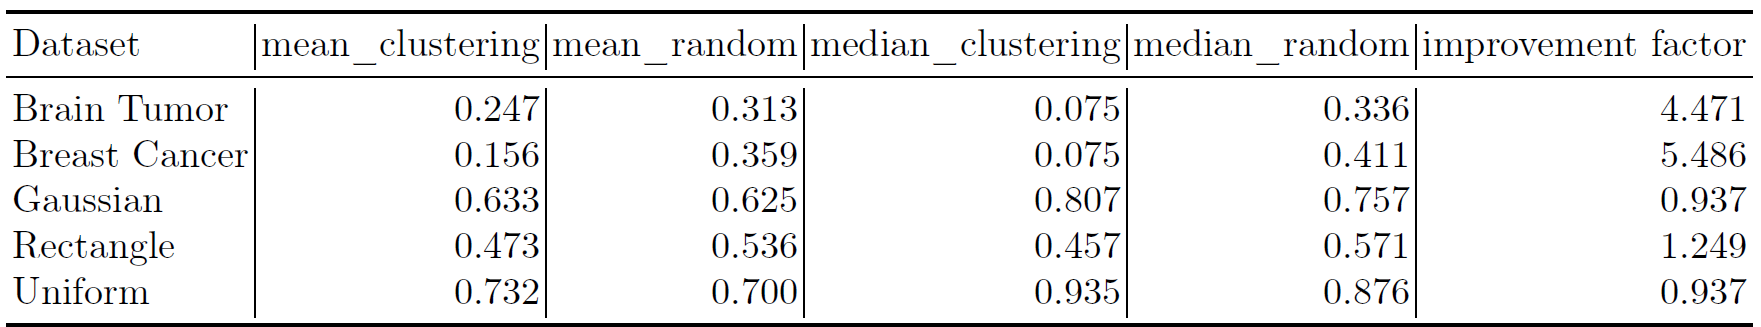
\includegraphics[width=1\linewidth]{score_df.png}
\end{figure}
Մեր մոտեցումը հանեգնում է միջինում նոր ձևով սահմանված անորոշության \textbf{2.61} անգամ նվազեցման
\end{frame}

\begin{figure}
\begin{figure}
    \makebox[\textwidth][c]{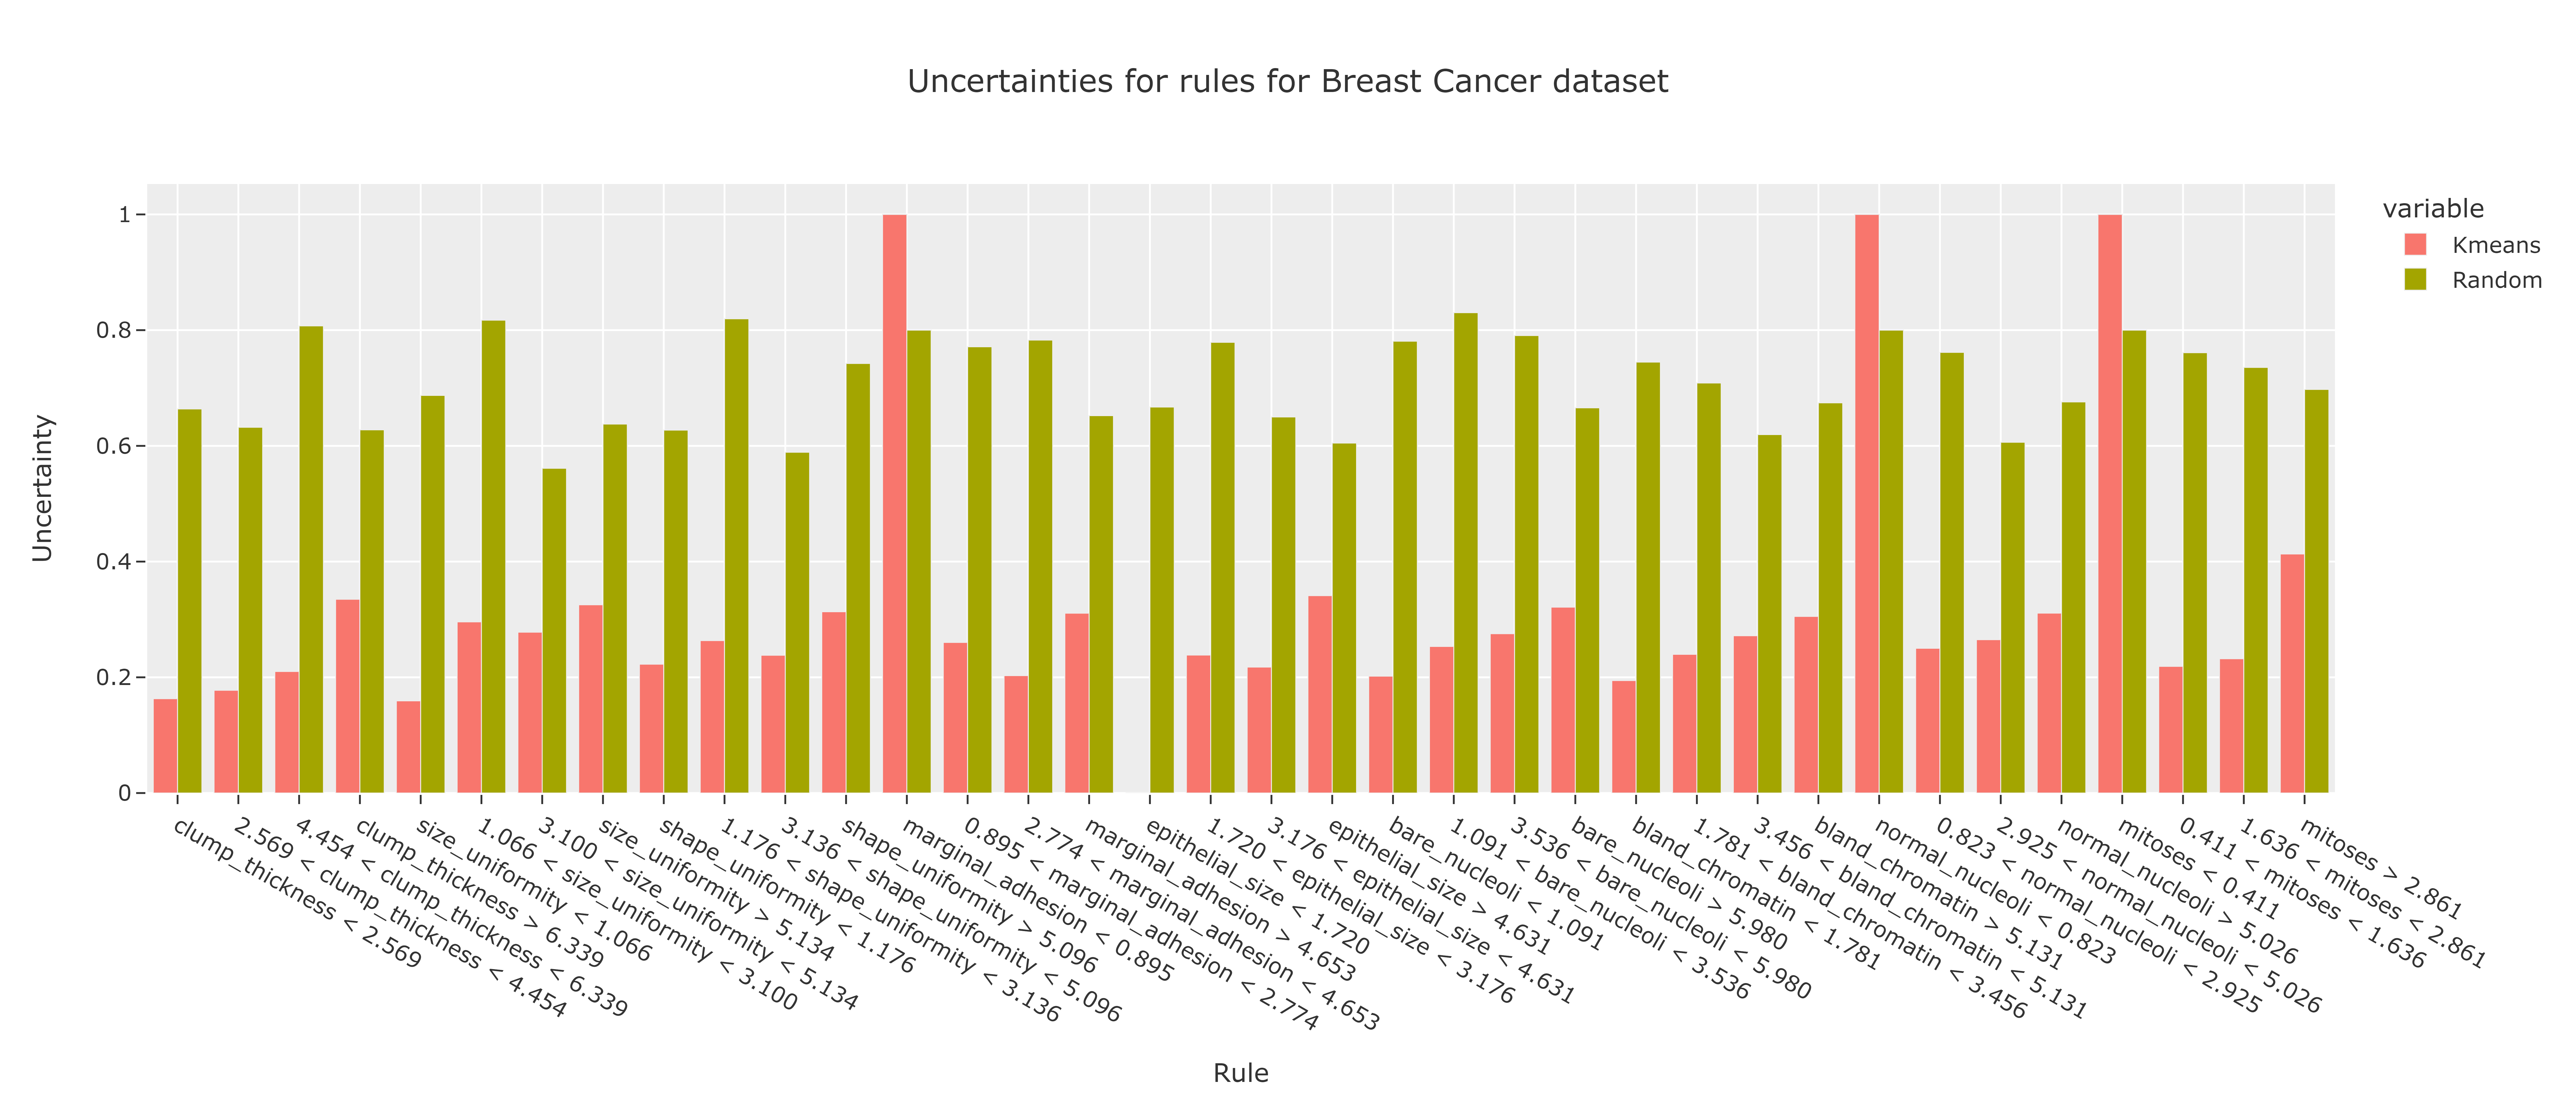
\includegraphics[width=\linewidth]{bars.png}} 
    \caption{Ըստ { \rm MAF initialization}-ի անորոշությունները տարատեսակ օրենքների համար}
    \label{fig:bars}
\end{figure}
\end{figure}

\begin{frame}{Գրականություն}
    
\begin{thebibliography}{8}
{\rm
\bibitem{dst}
Shafer, G.: A Mathematical Theory of Evidence. Princeton University Press, Princeton (1976)

\bibitem{sergio}
Peñafiel, S., Baloian, N., Sanson, H., \& Pino, J. A.: Applying Dempster–Shafer theory for developing a flexible, accurate and interpretable classifier. Expert Systems with Applications \textbf{148}, 113262 (2020)

\bibitem{kmeans}
J. MacQueen . Some methods for classification and analysis of multivariate observations. Proc. Fifth Berkeley Symp. on Math. Statist. and Prob., Vol. 1 (Univ. of Calif. Press, ), 281--297. (1967)

\bibitem{breastCancer}
Wolberg, W. H., Mangasarian, O. L.: Multisurface method of pattern separation for medical diagnosis applied to breast cytology. Proceedings of the National Academy of Sciences \textbf{87}(23), 9193--9196 (1990)

\bibitem{brainTumor}
Bohaju, J.: Brain Tumor. In: Kaggle 2020, DOI: \doi{10.34740/KAGGLE/DSV/1370629}. \url{https://www.kaggle.com/dsv/1370629} (2020)
}
\end{thebibliography}
\end{frame}

\begin{frame}
\begin{figure}
    \centering
    
\includegraphics[scale=0.27]{AUA_Codassca2024_website-100-2048x596.jpg}
\end{figure}
    
\end{frame}

\begin{frame}
    \begin{center}
        \Huge Շնորհակալություն
    \end{center}
\end{frame}


\end{document}


% ToDO if have time
% \section{SHAP Interpretability}
% \begin{frame}{SHAP Interpretability: A Mathematical View}
%   \begin{itemize}
%     \item \textbf{Objective:} SHAP provides a unified measure of feature importance based on Shapley values from cooperative game theory.
%     \item \textbf{Process:}
%       \begin{enumerate}
%         \item Calculate the contribution of each feature to the prediction by considering all possible combinations of features.
%         \item This involves computing the difference in the model's prediction with and without the feature, averaged over all possible subsets of features.
%       \end{enumerate}
%     \item \textbf{Mathematical Formulation:}
%       \begin{itemize}
%         \item Let \( f \) be the prediction model, \( x \) be the instance to explain, and \( S \subseteq F \setminus \{i\} \) where \( F \) is the set of all features and \( i \) is a feature.
%         \item The SHAP value \( \phi_i \) for feature \( i \) is given by:
%           \[
%           \phi_i(f, x) = \sum_{S \subseteq F \setminus \{i\}} \frac{|S|! (|F| - |S| - 1)!}{|F|!} [f_x(S \cup \{i\}) - f_x(S)]
%           \]
%         \item Here, \( f_x(S) \) is the prediction of model \( f \) with features in set \( S \) active, and the term outside the brackets is a weight representing the number of ways to form \( S \).
%       \end{itemize}
%     \item \textbf{Interpretation:} SHAP values explain the prediction of instance \( x \) by quantifying the contribution of each feature to the difference between the actual prediction and the average prediction.
%   \end{itemize}
% \end{frame}



